Radial distribution networks are the most common type of distribution networks and are characterized by a tree-like structure that branches out from a central source to various customers. Power flows in a single direction from the source to the loads. \cite{PowerSystemAnalysis:1994}

\begin{figure}[h]
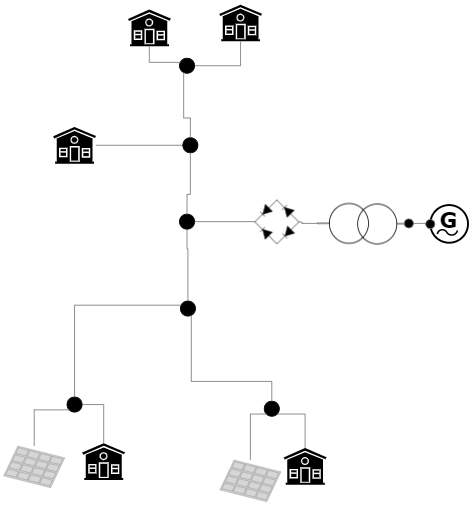
\includegraphics{Radial distribution network.png}
\label{fig:Radial distribution network}
\caption{Radial distribution network}
\end{figure}



\begin{comment}

potential sources
[2] T.A. Short, Power System Stability and Control, IEEE Press, 1993.
[3] J.K. Saini and P. Kundur, Power System Stability and Control, CRC Press, 2007.
[4] R. Lasseter and G. Andhankar, "Microgrids and Active Distribution Networks," IEEE Power and Energy Magazine, vol. 11, no. 3, pp. 40-50, 2013.
\end{comment}